% !TEX root = ../main.tex
% --+ 11.41 SUMMARY +-----------------------------------------------------------
\begin{frame}{FMT Efficiency}
    \label{11.41::summary}
    \begin{itemize}
        \item
            Initially, my plan was to work with run \ef{12933} (10.4 GeV beam, 250 nA), but analysis shows a very poor FMT efficiency.

        \item
            This issue comes from three sources: \ef{alignment}, \ef{reconstruction}, and \ef{geometry}.
    \end{itemize}

    \vspace{-12pt}
    \begin{columns}[onlytextwidth,T]

    \begin{column}{.05\linewidth}\end{column} % Centering column.

    \begin{column}{.49\linewidth}
        \begin{center}
            \begin{figure}[t]
                \centering{
                    \fbox{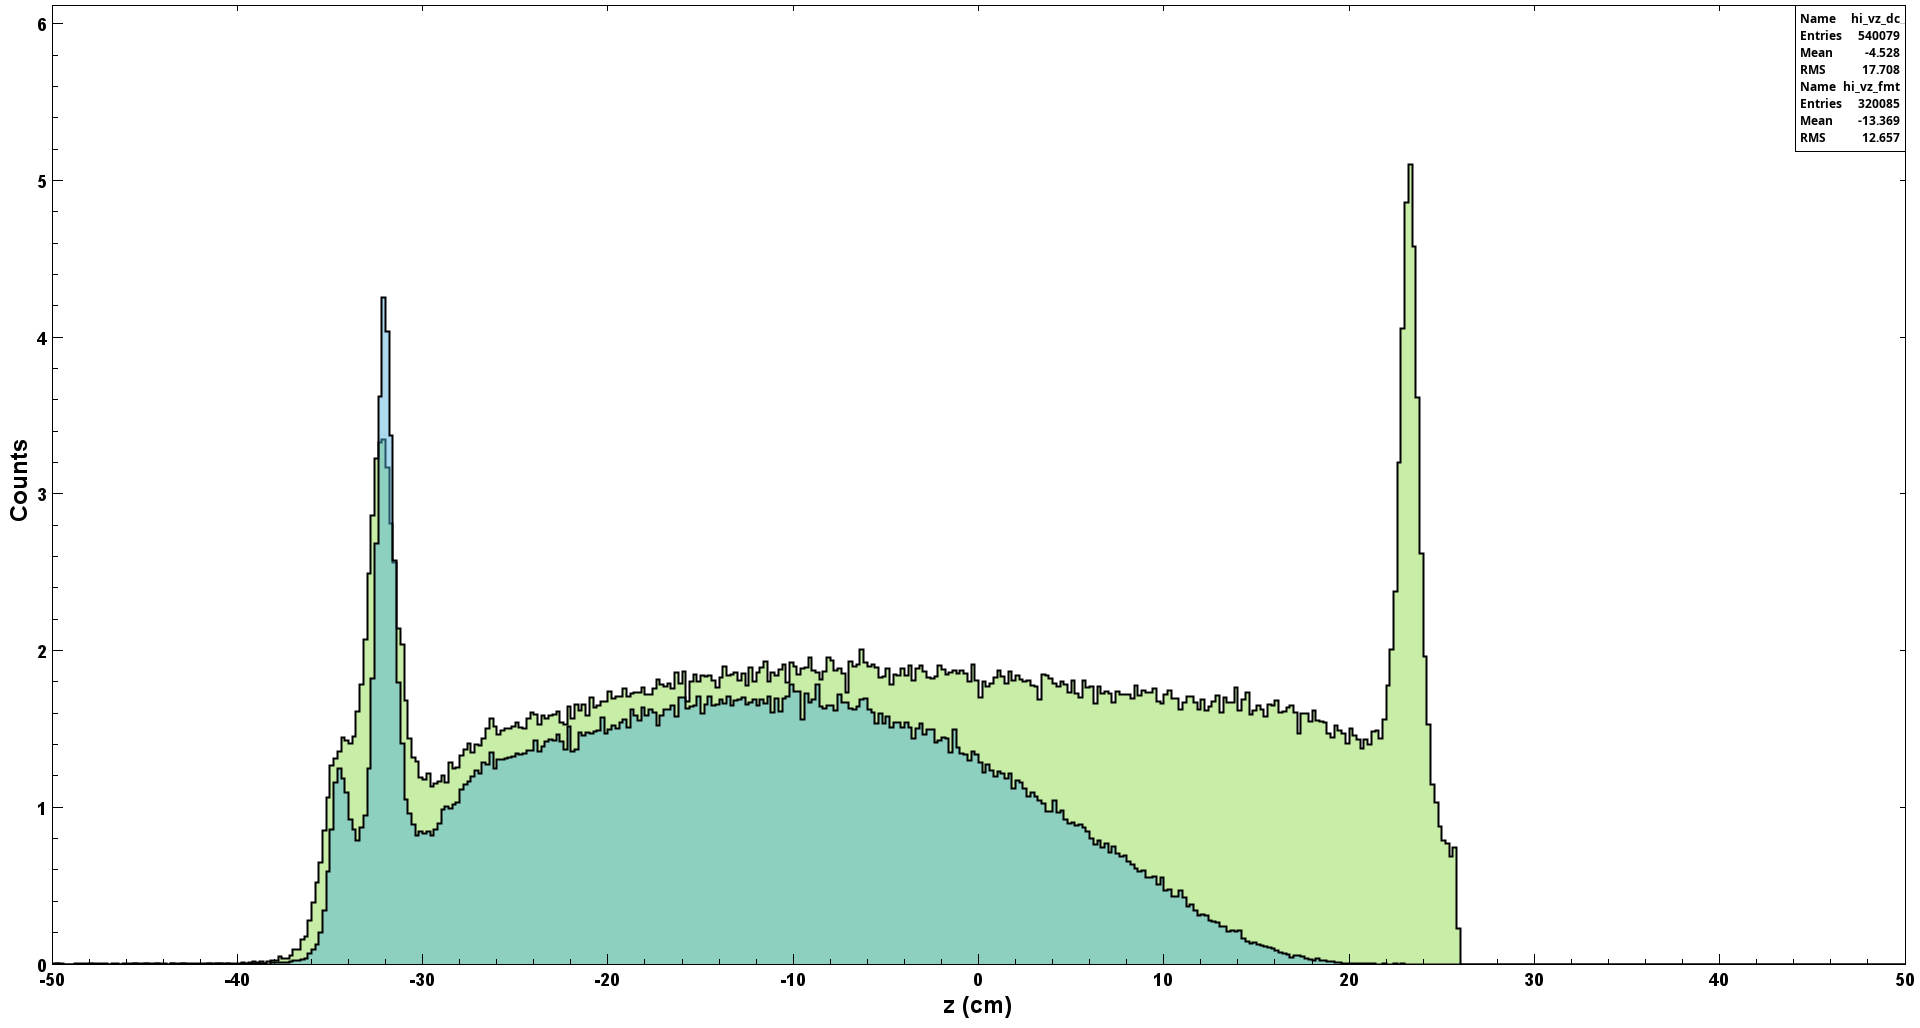
\includegraphics[width=\textwidth]{41vz_011983.png}}
                }
                \textit{Run \ef{11983}, reconstructed in 2020.}
            \end{figure}
        \end{center}
    \end{column}

    \begin{column}{.29\linewidth}
        \begin{center}
            \begin{figure}[t]
                \centering{
                    \fbox{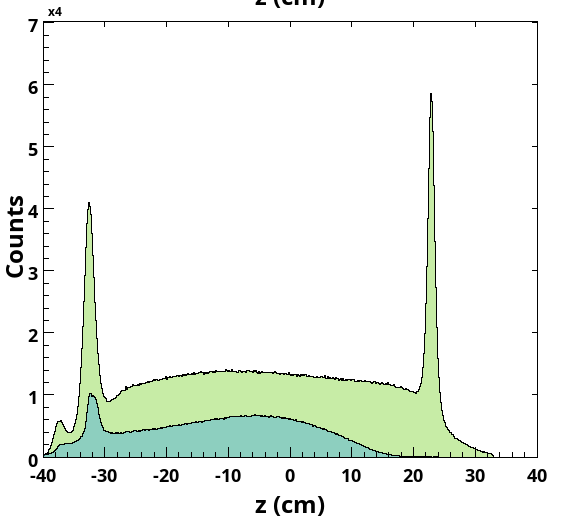
\includegraphics[width=\textwidth]{41vz_012933.png}}
                }
                \textit{Run \ef{12993}, 2023.}
            \end{figure}
        \end{center}
    \end{column}

    \begin{column}{.05\linewidth}\end{column} % Centering column.

    \end{columns}
    \begin{center}
        \textit{\ef{$v_z$} for \textbf{\textcolor[HTML]{c7eca6}{DC (green)}} and \textbf{\textcolor[HTML]{8dcfbf}{FMT (cyan)}} tracks.}
    \end{center}
\end{frame}

